%%%%%%%%%%%%%%%%%%%%%%%%%%%%%%%%%%%%%%%%%%%%%%%%%%%%%%%%%%%%%%%%%%%%%%%%%%%%%%%%
% Thesis / Project Report
% LaTeX Template
% Version 2.0 (08/04/16)
%
% Author:
% Siddhant Shrivastava
% https://github.com/sidcode/bits-pilani-thesis-template-latex
%
% This template is heavily based on the work of Darshit Shah, Steven Gunn and Sunil Patel
% Darshit Shah
% https://github.com/darnir/BPHC-LaTeX-Report-Class
% Steven Gunn
% http://users.ecs.soton.ac.uk/srg/softwaretools/document/templates/
% and
% Sunil Patel
% http://www.sunilpatel.co.uk/thesis-template/
%
% License:
% CC BY-NC-SA 4.0 (http://creativecommons.org/licenses/by-nc-sa/4.0/)
%
% Note:
% Make sure to edit document variables in the Thesis.cls file
%
%%%%%%%%%%%%%%%%%%%%%%%%%%%%%%%%%%%%%%%%%%%%%%%%%%%%%%%%%%%%%%%%%%%%%%%%%%%%%%%%

%-------------------------------------------------------------------------------
%	PACKAGES AND OTHER DOCUMENT CONFIGURATIONS
%-------------------------------------------------------------------------------

\documentclass[11pt, a4paper, oneside]{Thesis} % Paper size, default font size
                                               % and one-sided paper

\graphicspath{{Pictures/}} % Specifies the directory where pictures are stored

% \usepackage{lineno} 
% \linenumbers % TODO: Line numbers in draft mode. Disable before submitting

% \usepackage[sfdefault]{atkinson} % atkinson hyperlegible font

\usepackage[backend=bibtex]{biblatex} % bibliography in the end
\bibliography{bibliography}

\usepackage{nameref}
\usepackage{minted}

\title{\ttitle} % Defines the thesis title - don't touch this

\begin{document}

\frontmatter % Use roman numbering style (i, ii...) for the pre-content pages

\setstretch{1.3} % Line spacing of 1.3

% Define page headers using FancyHdr package and set up for one-sided printing
\fancyhead{} % Clears all page headers and footers
\rhead{\thepage} % Sets the right side header to show the page number
\lhead{} % Clears the left side page header

\pagestyle{fancy} % Finally, use the "fancy" page style to implement the
                  %FancyHdr headers

% Input all the variables used in the document. Please fill out the
% variables.tex file with all your details.
%-------------------------------------------------------------------------------
%	DOCUMENT VARIABLES
%
%	Fill in the lines below to set the various variables for the document
%-------------------------------------------------------------------------------

%-------------------------------------------------------------------------------
% Your thesis title - this is used in the title and abstract
% Command: \ttitle
\thesistitle{Atmosphere and the TCP/IP Stack for Maximizing Security}
%-------------------------------------------------------------------------------
% The document type: Thesis / report, etc.
% Command: \doctype
\documenttype{Undergraduate Thesis}
%-------------------------------------------------------------------------------
% Your supervisor's name - this is used in the title page
% Command: \supname
\supervisor{Dr. Anton Burtsev}
%-------------------------------------------------------------------------------
% The supervisor's position - Used on Certificate
% Command: \suppos
\supervisorposition{Associate Professor}
%-------------------------------------------------------------------------------
% Supervisor's institute
% Command: \supinst
\supervisorinstitute{University of Utah}
%-------------------------------------------------------------------------------
% Your Co-Supervisor's name
% Command: \cosupname
\cosupervisor{Dr. K Hari Babu}
%-------------------------------------------------------------------------------
% Co-Supervisor's Position - Used on Certificate
% Command: \cosuppos
\cosupervisorposition{Asst. Professor}
%-------------------------------------------------------------------------------
% Co-Supervisor's Institute
% Command: \cosupinst
\cosupervisorinstitute{BITS Pilani Pilani Campus}
%-------------------------------------------------------------------------------
% Your Examiner's name. Not currently used anywhere.
% Command: \examname
\examiner{}
%-------------------------------------------------------------------------------
% Name of your degree
% Command: \degreename
\degree{Bachelor of Engineering (Hons.)}
%-------------------------------------------------------------------------------
% The BITS Course Code for which this report is written
% COmmand: \ccode
\coursecode{BITS F421T}
%-------------------------------------------------------------------------------
% The name of the Course
% Command: \cname
\coursename{Thesis}
%-------------------------------------------------------------------------------
% Your name. Extend manually in case of multiple authors
% Command: \authornames
\authors{Tirth Jain}
%-------------------------------------------------------------------------------
% Your ID Number - used on the Title page and abstract
% Command: \idnum
\IDNumber{2019A7TS0120P}
%-------------------------------------------------------------------------------
% Your address
% Command: \addressnames
\addresses{}
%-------------------------------------------------------------------------------
% Your subject area
% Command: \subjectname
\subject{}
%-------------------------------------------------------------------------------
% Keywords for this report.
% Command: \keywordnames
\keywords{Microkernels, Networking, Fault Isolation, TCP/IP}
%-------------------------------------------------------------------------------
% University details
% Command: \univname
\university{\texorpdfstring{\href{http://www.bits-pilani.ac.in/} % URL
                {Birla Institute of Technology and Science Pilani}} % University name
                {Birla Institute of Technology and Science Pilani}}
%-------------------------------------------------------------------------------
% University details, in Capitals
% Command: \UNIVNAME
\UNIVERSITY{\texorpdfstring{\href{http://www.bits-pilani.ac.in/} % URL
                {BIRLA INSTITUTE OF TECHNOLOGY AND SCIENCE PILANI}} % name in capitals
                {BIRLA INSTITUTE OF TECHNOLOGY AND SCIENCE PILANI}}

%-------------------------------------------------------------------------------
% Campus Name
% Command: \campusname
\campus{Pilani Campus}

%-------------------------------------------------------------------------------
% Campus Name, in capitals
% Command: \CAMPUSNAME
\CAMPUS{PILANI CAMPUS}


%-------------------------------------------------------------------------------
% Department Details
% Command: \deptname
\department{\texorpdfstring{\href{http://www.bits-pilani.ac.in/pilani/computerscience/ComputerScience} % Your department's URL
                {Computer Science \& Information Systems}} % Your department's name
                {Computer Science}}
%-------------------------------------------------------------------------------
% Department details, in Capitals
% Command: \DEPTNAME
\DEPARTMENT{\texorpdfstring{\href{http://www.bits-pilani.ac.in/pilani/computerscience/ComputerScience} % Your department's URL
                {COMPUTER SCIENCE \& INFORMATION SYSTEMS}} % Your department's name in capitals
                {COMPUTER SCIENCE \& INFORMATION SYSTEMS}}
%-------------------------------------------------------------------------------
% Research Group Details
% Command: \groupname
\group{\texorpdfstring{\href{https://mars-research.github.io/}
                {Mars Research}} % Your research group's name
                {Mars Research}}
%-------------------------------------------------------------------------------
% Research Group Details, in Capitals
% Command: \GROUPNAME
\GROUP{\texorpdfstring{\href{https://mars-research.github.io/}
                {MARS RESEARCH}}
                {MARS RESEARCH}}
%-------------------------------------------------------------------------------
% Faculty details
% Command: \facname
\faculty{\texorpdfstring{\href{https://www.cs.utah.edu/~aburtsev/index.html}
                {Anton Burtsev}}
                {Anton Burtsev}}
%-------------------------------------------------------------------------------
% Faculty details, in Capitals
% Command: \FACNAME
\FACULTY{\texorpdfstring{\href{Faculty Web Site URL Here (include http://)}
                {ANTON BURTSEV}}
                {ANTON BURTSEV}}
%-------------------------------------------------------------------------------


%-------------------------------------------------------------------------------
%   NON-CONTENT PAGES
%-------------------------------------------------------------------------------
\maketitle
\Declaration
\Certificate

% \Quotation{Insert Random Quote here. Publish like a boss.}{Your Name}

\begin{abstract}
Even after decades of work to make monolithic kernels more secure, serious vulnerabilities in them are still reported every year. Because the entire monolithic kernel is in one address space, an attacker is just one vulnerability away from owning the entire machine. We argue that it is time to decompose monolithic kernels like Linux into smaller parts that run in isolated compartments and communicate using secure interfaces. We think this is timely due to growing hardware and software support of isolation.

In this Thesis, I discuss Atmosphere, our approach to microkernelization and fault isolation of an operating system kernel. Specifically, my work focuses on the network stack which is part of our larger effort to build a new operating system, Atmosphere. We argue that the network stack is a source for bugs and that isolation is the way forward to minimize the impact of these bugs. 
\end{abstract}

% \begin{acknowledgements}
% Thanks to Anton for calling me to Utah and giving me this opportunity. Thanks to Prof. Hari Babu for teaching me NetProg. Thanks to Xiangdong for dragging me to the gym everyday and all of his compilers. Thanks to Zhaofeng for all the Nix shells and gatekeeping all our code. Without all of them, this Thesis wouldn't have been possible.
% \end{acknowledgements}

%-------------------------------------------------------------------------------
%	LIST OF CONTENTS/FIGURES/TABLES PAGES
%-------------------------------------------------------------------------------

% The page style headers have been "empty" all this time, now use the "fancy"
% headers as defined before to bring them back
\pagestyle{fancy}

\lhead{\emph{Contents}} % Set the left side page header to "Contents"
\tableofcontents % Write out the Table of Contents

% Set the left side page header to "List of Figures"
\lhead{\emph{List of Figures}}
% \listoffigures % Write out the List of Figures

 % Set the left side page header to "List of Tables"
\lhead{\emph{List of Tables}}
% \listoftables % Write out the List of Tables

%%-------------------------------------------------------------------------------
%%	ABBREVIATIONS
%%-------------------------------------------------------------------------------

%\clearpage % Start a new page

% % Set the line spacing to 1.5, this makes the following tables easier to read
%\setstretch{1.5}

%\lhead{\emph{Abbreviations}} % Set the left side page header to "Abbreviations"
%\listofsymbols{ll} % Include a list of Abbreviations (a table of two columns)
%{
%\textbf{LAH} & \textbf{L}ist \textbf{A}bbreviations \textbf{H}ere \\
%%\textbf{Acronym} & \textbf{W}hat (it) \textbf{S}tands \textbf{F}or \\
%}

%-------------------------------------------------------------------------------
%	PHYSICAL CONSTANTS/OTHER DEFINITIONS
%-------------------------------------------------------------------------------

% \clearpage % Start a new page

% % Set the left side page header to "Physical Constants"
% \lhead{\emph{Physical Constants}}

%  % Include a list of Physical Constants (a four column table)
% \listofconstants{lrcl}
% {
% Speed of Light & $c$ & $=$ & $2.997\ 924\ 58\times10^{8}\ \mbox{ms}^{-\mbox{s}}$ (exact)\\
% % Constant Name & Symbol & = & Constant Value (with units) \\
% }

%%-------------------------------------------------------------------------------
%%	SYMBOLS
%%-------------------------------------------------------------------------------

%\clearpage % Start a new page

%\lhead{\emph{Glossary}} % Set the left side page header to "Symbols"

%\listofnomenclature % List the nomenclature. (We use the glossaries package)

%-------------------------------------------------------------------------------
%	DEDICATION
%-------------------------------------------------------------------------------

\setstretch{1.3} % Return the line spacing back to 1.3

\pagestyle{empty} % Page style needs to be empty for this page

% Dedication text
% \Dedicatory{Dedicated to Kenkin, the emotional support capybara.}

\addtocontents{toc}{\vspace{2em}} % Add a gap in the Contents, for aesthetics

%-------------------------------------------------------------------------------
%	THESIS CONTENT - CHAPTERS
%-------------------------------------------------------------------------------

\mainmatter % Begin numeric (1,2,3...) page numbering

\pagestyle{fancy} % Return the page headers back to the "fancy" style

% Include the chapters of the thesis as separate files from the Chapters folder
% Uncomment the lines as you write the chapters

% Chapter 1

\chapter{Introduction} % Main chapter title

\label{Chapter1} % For referencing the chapter elsewhere, use \ref{Chapter1} 

\lhead{Chapter 1. Introduction} % This is for the header on each page - perhaps a shortened title

Operating system reliability is a topic that has been studied for decades but nevertheless remains a major concern today. Even thought its been 30 years since Linux kernel was developed, critical vulnerabilities are being found in the kernel. On top of that, the monolithic design (i.e., everything in the kernel is running in a single address space) makes it such that the attacker is only one exploit away from taking control of the entire system. This is concerning because device drivers, often developed by third parties are a major source of vulnerabilities. Redundancy in hardware and software protection mechanisms can protect against transient faults but persistent faults because of undetected logic flaws still remain a major concern. In recent times, with the advent of cloud services, this becomes even more significant because clouds often have to run untrusted code that needs to be isolated from other parts of the operating system.

Logic errors and faults can propogate from within a component and propogate to other parts of the system. Microkernelization aims to solve this problem by isolating various parts of an operating system and minimizing the effect of failures in a single subsystem. In a microkernel, only the bare minimum that is required to boot an operating system is included in the kernel. All other components such as the filesystem, the device drivers, and the network stack are run in separate isolated processes that interact with each other using some form of IPC. Inter component fault propogation can thus be reduced by introducing safe IPC mechanisms.

Atmosphere is a microkernel based operating system. In this thesis, I discuss the design of Atmosphere mainly focusing on the the network stack and how its design can be used to model other services of the operating system. The network stack was built with two main principles in mind: maximizing fault isolation and minimizing its cost on performance. For the first principle, we take microkernelization to its extremes and build a per connection (or per socket for UDP) network stack. This means, every new connection has its own TCP/IP stack that can process and dispatch packets. This ensures that if one connection is corrupted, the rest of the connections on the system can keep operating. Although this is not completely possible since there is some inherent shared state on any host machine on a network. In later sections we discuss how we minimize this shared state. For the second principle, we implement a zero copy model and explain how using Rust's guarantees help us implement this with confidence. On failure, a component can be safely restarted and meanwhile, all IPC calls to it can return an error. 

The rest of this Thesis is organised as follows: 

\begin{itemize}
    \item{In \nameref{Chapter2} and \nameref{Chapter3} we discuss modern primitives for software isolation and contemporary microkernels.}
    \item{\nameref{Chapter4} talks about the API design and the internals of the network stack we built. }
    \item{\nameref{Chapter5} evaluates the performance of the network stack as compared to the current standards. }
\end{itemize}

% Chapter Template

\chapter{Background and Related Work}

\label{Chapter2}

\lhead{Chapter 2. \emph{Backround and Related Work}} 

\tirth{some intro here? idk}

\section{Theseus}
Theseus\cite{theseus} is a microkernel based operating system written in Rust. Rust's safety guarantees enable Theseus to run all software written in Rust, including userspace applications, to run in a Single Address Space system with a Single Privilege level. Thus, eliminating the need for virtual memory management and protection rings. Theseus introduces the idea of cells that are described as a software-defined unit of modularity that serves as the core building block of the OS. A cell can be modeled as a crate in Rust. On booting, only the microkernel, ie, the \lstinline{nano_core} is loaded which bootstraps the system. All other cells are dynamically loaded on demand. 
Theseus piggybacks on Rust's safety guarantees to enable reliable IPC between cells. For example, memory mappings are a 1-1 mapping to a physical frame. They can only be shared behind a read-only \lstinline{&MappedPages} reference eliminating the double-free and the use-after-free problem. 

The most important contribution by Theseus is the idea of eliminating (or minimizing) shared state between components. All OS services can be modelled as servers and applications requesting these services are modelled as clients. Theseus eliminates state-spill\cite{state-spill} across cells by eliminating all state from the servers. Everything that is needed to service a client's request is stored in the client itself and thus the servers can be completely stateless. This allows a server cell to be replaced by a new cell without any state loss. This, however, is not always possible. In case a state cannot be eliminated, as in the case of descriptor tables, the state is stored in a \lstinline{state_db}. The \lstinline{state_db} is a key-value database that stores states with a static lifetime that the server can request a (weak) reference to. In case a server needs to be restarted, its state can be recovered from the \lstinline{statedb}. The statelessness of cells also allows for live updates. A server can be replaced, ie, a patch can be applied to a component without having to restart the entire operating system. Applying a patch is as simple as swapping a cell with a new cell.

\tirth{Maybe add limitations and performance evaluations of Theseus here?}

\section{Singularity OS}
Singularity\cite{singularity} introduced "Software Isolated Processes" which use software verification instead of hardware protection mechanisms to isolate processes. SIPs cannot have shared memory. Instead, data can be passed between SIPs using an "exchange heap". Data on the exchange heap can be owned only by a single process but the ownership can be "transferred". Static verification ensure that programs do not try to access an object after it has been passed (ie a dangling pointer). Ownership can be transferred between SIPs using "Contract-Based Channels". Channels are described using statically defined interfaces in the Sing# language. The communicating SIPs act as state machines with clearly defined states and the messages that can be passed on each state. Once a message has been passed, its data can no longer be used by the sending SIP. Ownership of data on the exchange heap is recorded so that blocks can be freed on process termination preventing memory leaks. This process isolation allows singularity to run the kernel and all SIPs in a single physical address space.

All programs running on Singularity must ship with a manifest. Manifest-based programs clearly define their resource requirements, desired capabilities and dependencies on other programs. The manifest can be used by the system to ensure that the program's requirements can be met and that the program satisfies all correct usage guarantees. The absence of shared memory and static verification of all communication makes the creation and termination of SIPs inexpensive.
\section{sel4}

\section{RedLeaf}


\chapter{Atmosphere Design}

\label{Chapter3}

\lhead{Chapter 3. \emph{Atmosphere Design}} 

\section{Safe IPC}

\tirth{Describe RedLeaf RRef interface.}

\chapter{The Network Stack} % Main chapter title

\label{Chapter4} % For referencing the chapter elsewhere, use \ref{Chapter1} 

\lhead{Chapter 4. The Network Stack} % This is for the header on each page - perhaps a shortened title

In this chapter, we take a look at how we implemented the UDP stack for Atmosphere. Since Atmosphere is not ready yet, we build a standalone network stack that runs in the userspace and evaluate its performance. We use a custom userspace network driver (based on Ixy) to process raw ethernet frames sent to and from the network stack. This driver is shared across applications just as it would be in the real Atmosphere.

\begin{figure}[!htbp]
	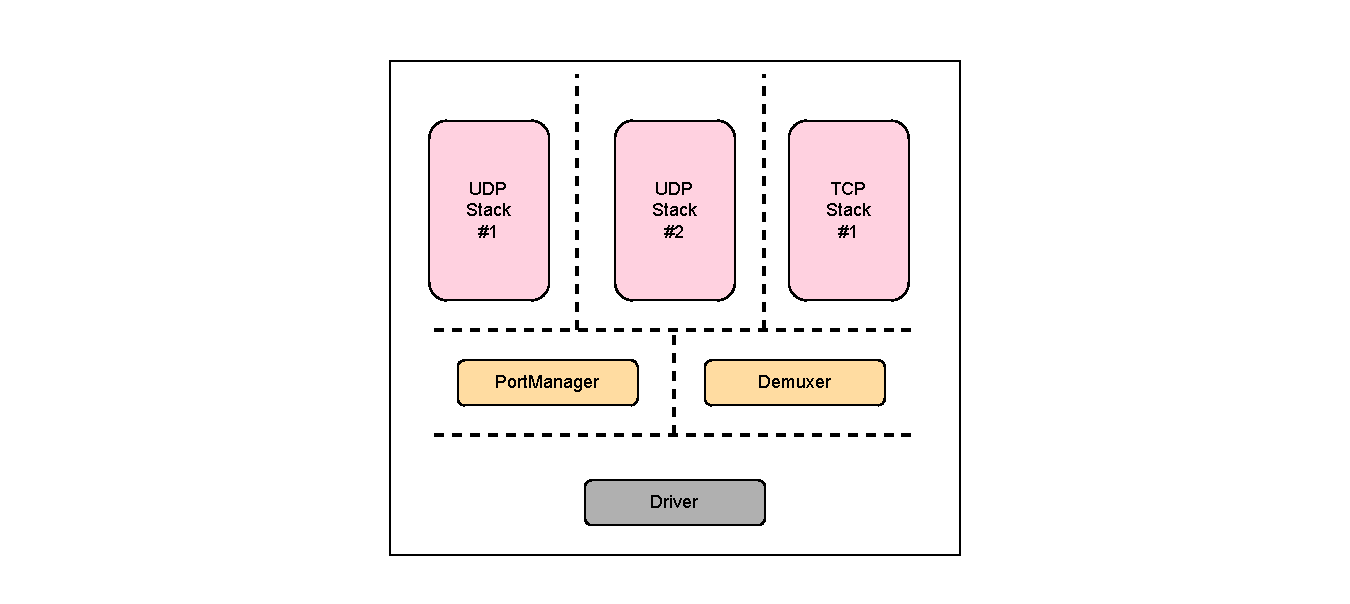
\includegraphics[width=1.0\columnwidth]{figures/network-design.pdf}
\caption{Atmosphere network stack design}
	\label{fig:network-design}
\end{figure}

\section{Driver for the Network Card}

Ixy is a network driver implemented in the userspace for Intel's Ixgbe family of network cards that shows how network cards work at the driver level. It is implemented in a fashion similar to DPDK and Snabb. We use a version of Ixy written in Rust and modify it to fit the design of our network stack. Two main limitations of Ixy (as per our design) are: (1) it handles allocations in the driver and (2) received packets cannot be reused as transmit packets. (2) is important as for a lot of applications (e.g. MICA), we want to be able to flip headers in a received packet and send it back to the client. 

The major modifications we make to ixy.rs are:
\begin{itemize}
    \item{Change the way packets are allocated. We get rid of the huge-pages backed Mempool and allow packets to be discretely allocated. DMA mapping is done for every packet. }
\item{Receive queues do not allocate packets themselves. Instead, the application supplies a batch of allocated buffers which is used to read packets from the NIC. This relieves the NIC from having to do any allocations. }
\end{itemize}

On testing with an Ixgbe NIC with a line rate of 10GB/s, we see no drop in performance after our modifications.

\subsection{Packet Storage}
As mentioned above, packets are stored in a DMA-mapped page-sized buffer. Listing \ref{listing:1} illustrates the Packet struct and how it is allocated. While allocating a page for each packet is wasteful in terms of memory, there is no discernible change in performance in processing packets. This also enables the NIC to interleave packets from different applications in the same queue without crossing any isolation boundaries.

\begin{listing}[!ht]
\begin{minted}[fontsize=\footnotesize, frame=lines, framesep=2mm]{Rust}
#[repr(C, align(PAGESZ))]
pub(crate) struct PacketBuffer {
    data: [u8; PAGESZ]
}

pub struct Packet {
    pub(crate) addr_virt: *mut u8,
    pub(crate) addr_phys: usize,
    pub(crate) len: usize,
    pub(crate) data: Box<PacketBuffer>,
}

pub fn alloc_pkt(len: usize) -> Option<Packet> {
    let mut buffer = Box::new(PacketBuffer{ data: [0;PAGESZ] });
    let addr_virt = buffer.data.as_mut_ptr();
    let mut p = Packet {
        data: buffer,
        addr_virt,
        len,
        addr_phys: 0,
    };
    match vfio_map_dma(p.addr_virt as usize, PAGESZ) {
        Ok(addr_phys) => {
            p.addr_phys = addr_phys;
            Some(p)
        }
        Err(e) => {
            error!("{}", e);

            None
        }
    }
}
\end{minted}
\caption{Packet storage in modified ixy}
\label{listing:1}
\end{listing}


\section{Port Manager}
The PortManager handles all allocations and deallocations of ports and keeps track of which stacks they are bound to. To be able to formally verify its implementation in the future, the interface it exposes is minimal and it only interacts with the opaque identifiers rather than actual types. 
UDP stacks can be identified by using only the destination port in an incoming packet (we assume that the device is connected to a single IPv4 interface for simplicity). But for TCP connections, since a single port can handle multiple connections, and every connection is handled by a different stack, we maintain a separate flow table for matching TCP connections.
The PortManager also helps the demuxer identify which stack a packet should go to, or if it is to be dropped.

\section{Demuxer}
The demuxer matches incoming packets with a destination stack and and returns free buffers from the NIC to the stack that owns them. The demuxer can also maintains private queues for applications that are not actively receiving packets but have incoming packets destined to them. 
On receiving a packet, the demuxer parses the protocol and the destination port (or the TCP 5-tuple) and use the PortManger to find the destination stack. If the packet is matched, we push it to the private queue. The next time the application calls receive, the private queue is emptied and the packets are returned to the stack. If the private queue for a stack is saturated, incoming packets are simply dropped.

\subsection{Packet Flipping}
Since the buffers for a receive call come from a stack, and since all packets received might not be destined to the same stack, the demuxer can flip a buffer from its private queue so that the application does not lose a free buffer to the demuxer. This is done by popping a buffer from a private queue and flipping it with the received buffer. The application can then get a free buffer in return for the buffer it contributed for the packet of another stack.

\subsection{UDP Interface}
We provide a low level interface for the application to interface applications with the udp protocol. We provide a \lstinline{UdpStack} interface that exposes two main methods: \lstinline{tx_batch()} and \lstinline{rx_batch()} both of which are non-blocking and interact with discrete packet buffers. Note that this is currently a low level interface requiring the user to setup a static arp table and routes in the ipv4 table themeselves. this can be changed in the future when the stack is integrated with atmosphere. We also provide a convenience function called \lstinline{prepare_batch()} that lets users provide a buffer and fills discrete packets with all required headers and the data from the given buffer. For ease of manipulating packet headers, we provide a \lstinline{UDPPacketRepr} representation which has setters and getters for protocol headers. \ref{listing:2} illustrates the code for a simple UDP echo server.

\begin{listing}[!htb]
\begin{minted}[fontsize=\footnotesize, frame=lines, framesep=2mm]{Rust}
pub fn main() {
    let mut stack = create_udp_stack(Ipv4Address::new(10, 0, 0, 2), 5000);
    let mut free_bufs: VecDeque<RawPacket> = VecDeque::with_capacity(NUM_PACKETS);
    let mut recv_batch: VecDeque<UdpPacketRepr> = VecDeque::with_capacity(NUM_PACKETS);
    let mut send_batch: VecDeque<UdpPacketRepr> = VecDeque::with_capacity(NUM_PACKETS);

    let mut num_recvd;

    loop {
        (num_recvd, recv_batch, free_bufs) = stack
            .recv_batch(recv_batch, free_bufs, BATCH_SIZE)
            .expect("failed to receive packets");
        recv_batch.drain(..num_recvd).for_each(|mut pkt| {
            // flip source and destination
            pkt.set_udp_packet(|mut udp| {
                let src = udp.get_source();
                let dst = udp.get_destination();
                udp.set_destination(src);
                udp.set_source(dst);
            });
            pkt.set_ip_packet(|mut ip| {
                let src = ip.get_source();
                let dst = ip.get_destination();
                ip.set_destination(src);
                ip.set_source(dst);
            });
            send_batch.push_back(pkt);
        });
        (send_batch, free_bufs) = stack
            .send_batch(send_batch, free_bufs)
            .expect("failed to sent packets");
    }
}
\end{minted}
\caption{Example UDP echo server}
\label{listing:2}
\end{listing}

\chapter{Evaluation} 

\label{Chapter5}

\lhead{Chapter 5. Evaluation} 

%\input{Chapters/Chapter6}
%\input{Chapters/Chapter7}

%-------------------------------------------------------------------------------
%	THESIS CONTENT - APPENDICES
%-------------------------------------------------------------------------------

\addtocontents{toc}{\vspace{2em}} % Add a gap in the Contents, for aesthetics

\appendix % Cue to tell LaTeX that the following 'chapters' are Appendices

% Include the appendices of the thesis as separate files from the Appendices
% folder
% Uncomment the lines as you write the Appendices

% % Appendix A

\chapter{Appendix Title Here} % Main appendix title

\label{AppendixA} % For referencing this appendix elsewhere, use \ref{AppendixA}

\lhead{Appendix A. \emph{Appendix Title Here}} % This is for the header on each page - perhaps a shortened title

Write your Appendix content here.

%\input{Appendices/AppendixB}
%\input{Appendices/AppendixC}

\addtocontents{toc}{\vspace{2em}} % Add a gap in the Contents, for aesthetics

\backmatter

%-------------------------------------------------------------------------------
%	BIBLIOGRAPHY
%-------------------------------------------------------------------------------

\label{Bibliography}

\lhead{\emph{Bibliography}} % Change the page header to say "Bibliography"

\printbibliography

\end{document}
